\section*{Introduction}

Lung adenocarcinoma (LUAD) is the most common subtype of lung cancer
and remains the leading cause of cancer death worldwide.\cite{herbst2018lung}
Treatment selection has become biomarker-conditional: targeted
therapy for \textit{EGFR}-mutant LUAD (osimertinib),\cite{soria2018flaura}
\textit{KRAS}\,G12C inhibition (sotorasib),\cite{skoulidis2021codebreak}
and immune-checkpoint blockade calibrated by
\textit{STK11}/\textit{KEAP1} co-mutation
status\cite{skoulidis2018stk11pd1} all require molecular profiling
that is logistically costly, slow, and unevenly available in
low- and middle-income settings.\cite{vanderlaan2018molecular}
H\&E-only mutation prediction directly from the digitised slide is
therefore an attractive triage tool---one that, in principle,
returns a per-gene answer in seconds at the cost of a scan.

% --- The published competition ---
A line of work pioneered by Coudray~et~al.\cite{coudray2018classification}
(Inception-v3 end-to-end, $n=382$, EGFR $\auroc=0.826$,
KRAS $\auroc=0.733$) and continued by
Kather~et~al.\cite{kather2020pancancer}, Saldanha~et~al.\cite{saldanha2023npj},
Logan~et~al.\cite{logan2022medrxiv} and most recently
Zhao~et~al.\cite{zhao2025deepgem} (DeepGEM MIL, $n=3{,}637$, AUROC
$0.82$--$0.96$), Campanella~et~al.\cite{campanella2025eagle}
(EAGLE, $n=8{,}461$, EGFR $\auroc=0.890$), and
Wang~et~al.\cite{wang2024chief} (CHIEF, $n=60{,}530$) has progressively
expanded both cohort size and the number of genes that can be called
above $\auroc=0.70$.
However, three problems remain unsolved by this trajectory:

\textbf{(1) Opacity at the level the pathologist uses.}
With a few exceptions, the published systems are
end-to-end CNN or MIL pipelines whose only output is a probability
per gene, optionally with an attention heatmap.
A heatmap shows \emph{where} the model is looking, not \emph{what}
it is seeing or \emph{why} that morphology should imply the
mutation; it cannot be argued against a textbook description of an
acinar gland or an invasive mucinous pattern, and it cannot be
edited by the pathologist.\cite{jain2019attention,rudin2019stop}
Clinical adoption demands an explanation that respects the WHO/IASLC
histological vocabulary in which pathologists already
reason.\cite{who2021thoracic,nicholson2022ialcslurp}

\textbf{(2) The cohort-mean metric hides per-gene structure.}
A typical paper reports a single cohort-average AUROC or a
gene-by-gene table without acknowledging that the genes themselves
sit on entirely different points of the H\&E-to-mutation pipeline:
some are predictable because the morphology is overt (TP53 high
nuclear pleomorphism), others because of a recurring \emph{pattern
combination} (KRAS via the invasive mucinous adenocarcinoma proxy,
which is morphologically lepidic$\,+\,$solid co-occurrence),
and others not because the signal lives in a stromal or biochemical
substrate that the LUAD pattern ontology does not encode (KEAP1's
NRF2 oxidative-stress axis; RBM10's splicing
defect).\cite{shim2015krasmucinous,rekhtman2013krassolid,cha2017imapatterns,li2011keap1papillary,bechara2013rbm10}
A method that wins on TP53 by 1~AUROC point may be losing on KEAP1
for an entirely orthogonal reason.

\textbf{(3) The cohort-scale arms race excludes most labs.}
EAGLE, CHIEF and the foundation-model line require
$10^4$--$10^5$ proprietary slides; a typical academic or hospital
laboratory has $10^2$--$10^3$.
Yet the public TCGA-LUAD release ($n=687$ usable slides after
quality filtering, $668$ patients) is still the most-cited
benchmark and is what most subsequent methods will be tested
against.\cite{tcga2014luad}
A pipeline that is honest about what is and is not predictable
\emph{from this cohort alone}, with a clear per-gene verdict, is
arguably more useful to the community than a foundation-scale
black box trained behind a paywall.

% --- Our contribution ---
This paper presents \lchai{}\,v2 (Lung Cancer Histologic Analysis
with Interpretable AI), a pattern-informed MIL system designed
against the three problems above.

% --- The conceptual frame: domain translation ---
Conceptually, we treat H\&E-based mutation prediction as an
\emph{imperfect translation between two clinical domains}: a
\emph{source} domain of tissue morphology and a \emph{target}
domain of somatic driver mutations.
To make the translation as faithful as the source permits, we first
render the morphology with the strongest available angular-margin
tile classifier---\fuzzyarc{}\,V2\cite{limareina2026fuzzyarc},
which attains the highest macro-F1 and, critically, the highest
per-class F1 on the ambiguous \emph{cribriform} boundary, the
hardest growth pattern to call.
Under this lens the six-pattern ANORAK ontology is the source
\emph{vocabulary}, the MIL aggregator is the \emph{translator}, and
the per-gene AUROC measures how much of the mutation ``language''
is expressible in morphological words.
The three-regime taxonomy (below) is then a statement about
\emph{translational faithfulness}: TP53/EGFR translate well, KRAS
requires a non-additive grammar (pattern co-occurrence), and
STK11/KEAP1/RBM10 are largely \emph{untranslatable} from H\&E
alone---bounded here to $\auroc\!\in\![0.6,0.72]$ with positive
sets as small as $n_+\!=\!37$.
This framing is not cosmetic: it connects our per-gene ceiling to a
broad family of medical cross-domain inference tasks---radiogenomics,
pathomics-to-genomics, retinal-to-cardiovascular and
ECG-to-function mapping---where faithfulness is set by the physics
of the source modality rather than by the estimator, a point we
develop in the Discussion.

\begin{figure}[ht!]
  \centering
  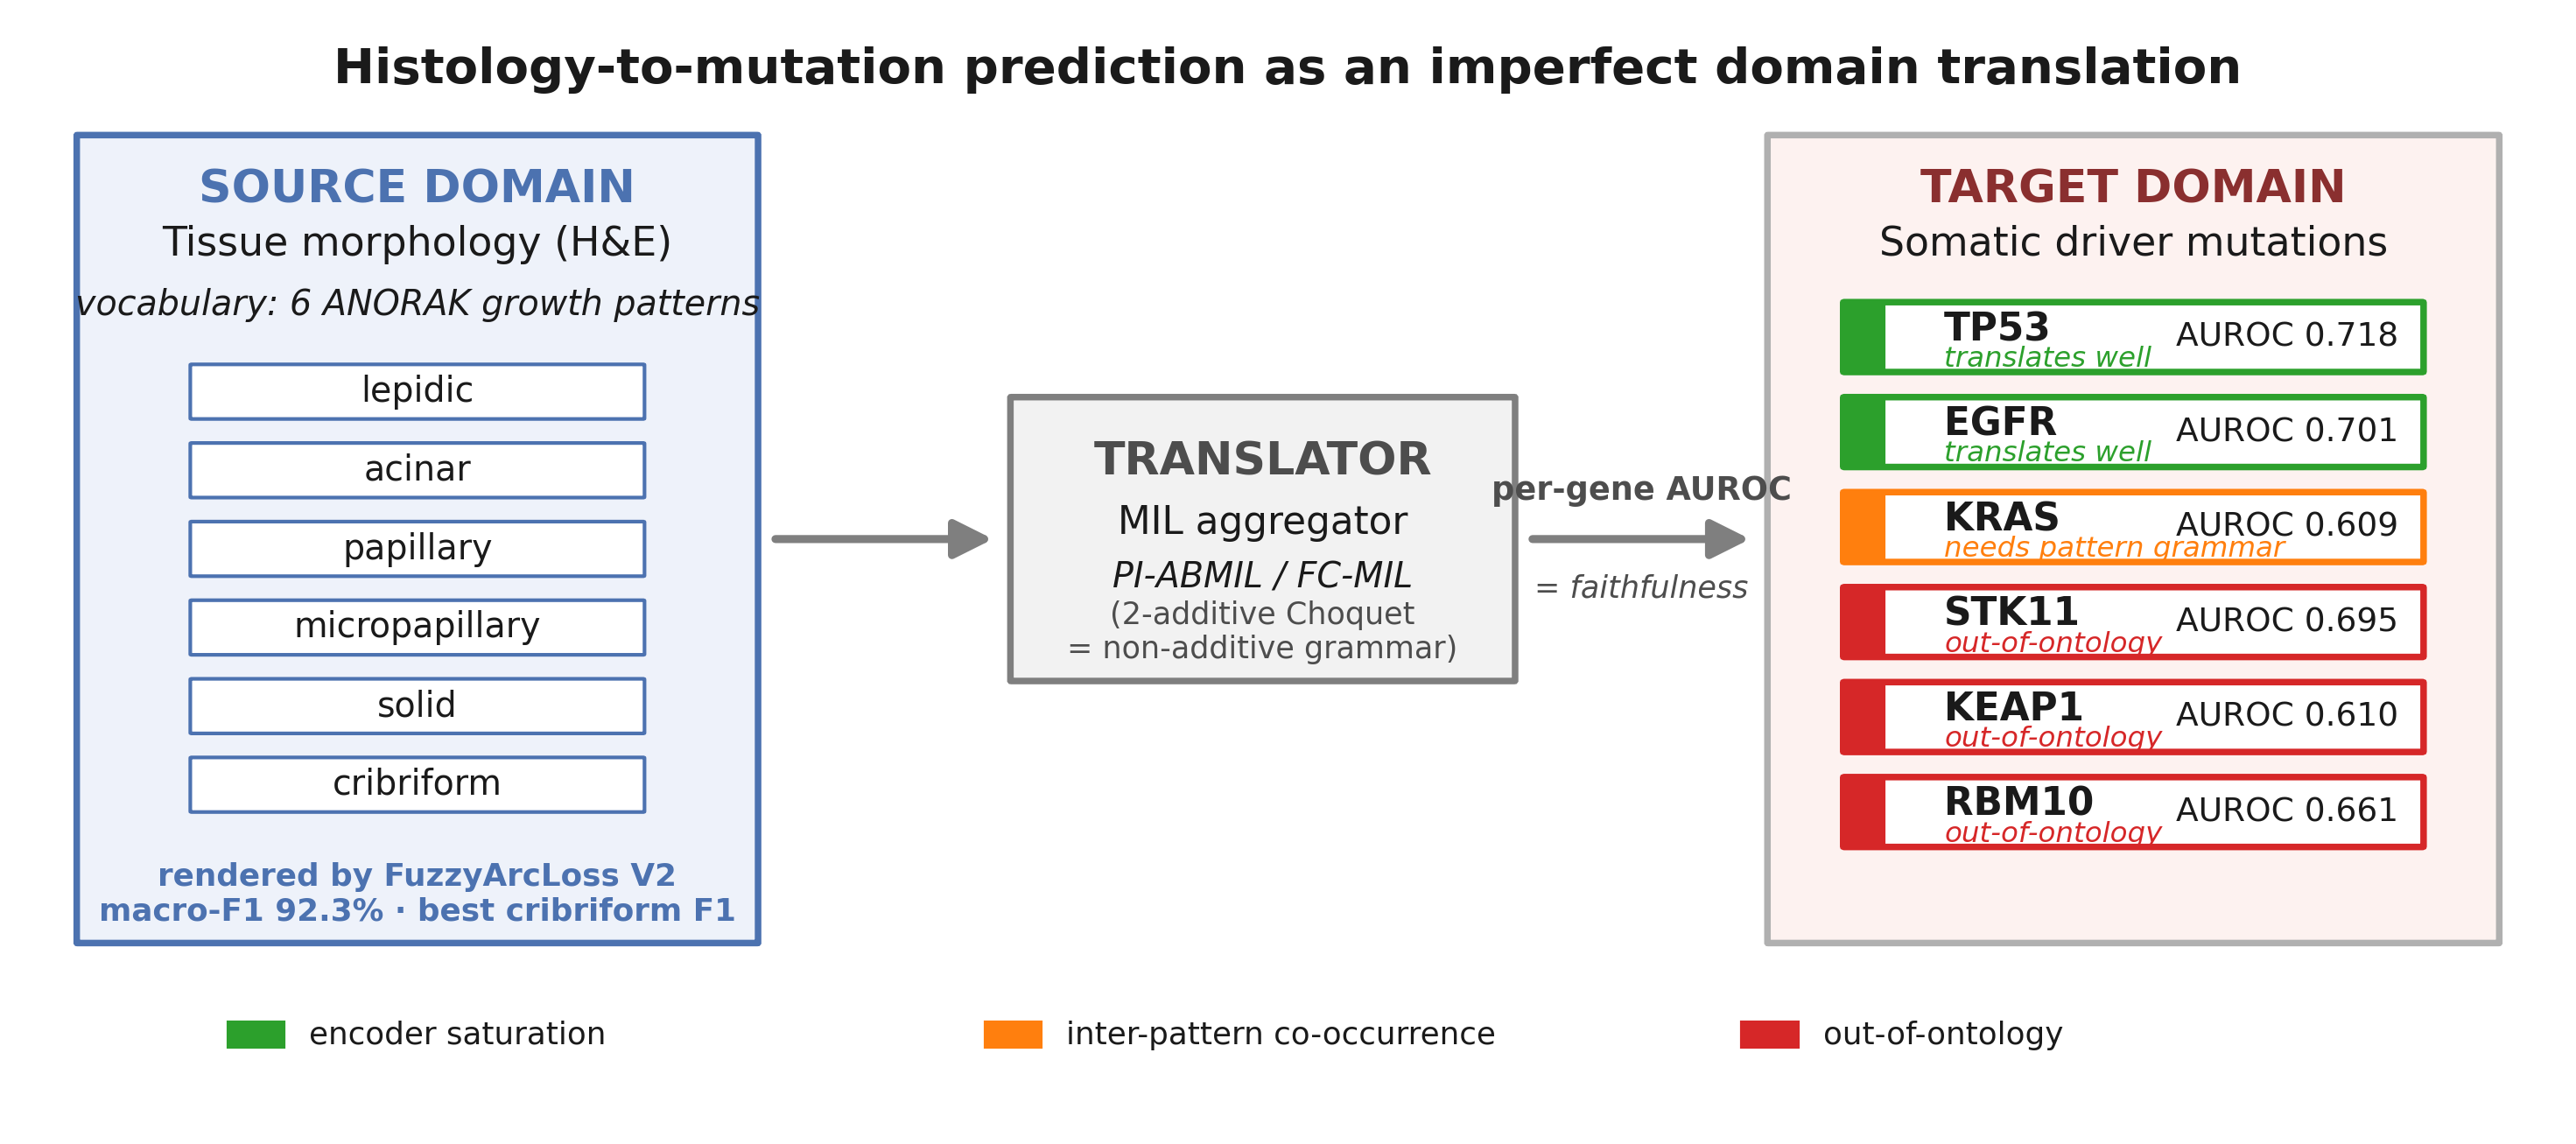
\includegraphics[width=\linewidth]{domain_translation_concept}
  \caption{\textbf{Histology-to-mutation prediction as an imperfect
  domain translation.} A \emph{source} domain of tissue morphology
  (H\&E), whose vocabulary is the six ANORAK growth patterns rendered
  by the \fuzzyarc{}\,V2 tile classifier\cite{limareina2026fuzzyarc}
  (macro-F1 $92.3\%$, best per-class F1 on the ambiguous cribriform
  boundary), is mapped by a MIL \emph{translator} (\piabmil{}/\fcmil{},
  the 2-additive Choquet integral supplying a non-additive grammar)
  onto a \emph{target} domain of somatic driver mutations. The
  per-gene AUROC measures translational faithfulness: TP53/EGFR
  translate well (encoder saturation), KRAS requires the non-additive
  grammar (inter-pattern co-occurrence), and STK11/KEAP1/RBM10 are
  largely untranslatable from H\&E alone (out-of-ontology).}
  \label{fig:domain_translation}
\end{figure}

Our contributions are:

\begin{itemize}
    \item \textbf{C1.\ A three-regime taxonomy that decomposes
    per-gene H\&E-based mutation predictability.}
    The six target genes partition into three qualitatively distinct
    regimes that answer \emph{why} the cohort-average AUROC is
    misleading.
    \emph{Regime~(i)~--~encoder saturation} (TP53, EGFR):\ the
    \ctranspath{} foundation encoder already saturates the
    predictable morphology and the 6-d categorical pattern channel
    adds no information ($\leq 0.02$ AUROC).
    \emph{Regime~(ii)~--~inter-pattern co-occurrence} (KRAS):\ a
    non-additive aggregator recovers a positive interaction index
    $I(\text{lepidic}\!\times\!\text{solid})\!=\!{+}0.032$ that
    matches the invasive mucinous adenocarcinoma proxy and that an
    additive concat-fusion attention head cannot express.
    \emph{Regime~(iii)~--~out-of-ontology} (STK11, KEAP1, RBM10):\
    the predictive signal lives outside the 6-pattern simplex---in
    the immune microenvironment (STK11), in a biochemical state with
    no consistent H\&E correlate (KEAP1), or below the class-prior
    collapse floor at $5\%$ prevalence (RBM10).
    The taxonomy is the central empirical contribution of the paper
    and tells the field where multimodal fusion (gene expression,
    radiology, micro-environment channels)---rather than another loss
    function or attention variant---is the natural next step for
    each gene.

    \item \textbf{C2.\ A six-level per-slide interpretability stack
    that exhibits the morphology-to-genotype translation.}
    We reframe interpretability from post-hoc attribution
    (\emph{where} the model looks) to \emph{translation made
    legible}: a bilingual account that renders each prediction in
    the source vocabulary (the six growth patterns) and, crucially,
    marks where the translation breaks down.
    For every slide and every gene we expose six interpretability
    layers derived from a single forward pass through the MIL
    aggregator:
    \textbf{L1}~MIL attention overlay (where the model is looking);
    \textbf{L2}~pattern overlay (what morphology it sees at each
    tile);
    \textbf{L3}~per-pattern SHAP decomposition;\cite{lundberg2017shap}
    \textbf{L4}~Choquet--Shapley intrinsic contribution and pairwise
    interaction indices (which pattern \emph{pairs} co-vote);
    \textbf{L5}~per-slide channel ablation ($\Delta\auroc$ per input
    channel);
    \textbf{L6}~fuzzy linguistic labels
    (\emph{very low / low / moderate / high / very high}) on every
    continuous score.
    Each level is clickable, editable, and can be argued against by
    the pathologist; together they act as the \emph{bilingual
    dictionary} that makes the translation---and its
    failures---inspectable (\emph{where + what + why}), which an
    attention heatmap alone cannot deliver.
    Under this view L4 (Choquet--Shapley) is the non-additive
    \emph{grammar} of the source language, and an Inconclusive verdict
    is reported as \emph{untranslatability} rather than as a silent
    low score.

    \item \textbf{C3.\ A per-gene Conclusive/Inconclusive verdict
    operationalising the three-regime taxonomy.}
    Cohort-level signal presence (mean AUROC $\geq 0.70$) is
    reported \emph{separately} from per-slide confidence (model
    probability), so a Conclusive verdict does not propagate into
    per-slide overclaim and an Inconclusive verdict does not suppress
    potentially useful per-slide ranking.
    The verdict is the operational artefact that surfaces Regime~(i)
    Conclusive (TP53, EGFR) versus Regimes~(ii)--(iii) Inconclusive
    (KRAS, STK11, KEAP1, RBM10) at the user-interface level.

    \item \textbf{C4.\ A dual anti-hallucination LLM explanation
    layer grounded in NCIt$+$MONDO.}
    The final step renders the translation into natural language:
    an LLM agent receives the structured slide-level evidence bundle
    from C2 and produces a clinical narrative.
    The fuzzy labels (L6) constrain \emph{how} it speaks (no spurious
    decimal precision; a probability of $0.59$ is reported as
    \emph{moderate}, not \emph{high})
    and a curated three-layer knowledge graph
    (NCIt~$+$~MONDO~$+$ dynamic-case$/$DeepSearch literature layer)
    acts as the \emph{target-domain lexicon}, constraining \emph{what}
    entities and edges the narrative may invoke so the translator
    cannot coin genotype ``words'' that do not exist.
    Deactivation-without-deletion records pathologist corrections as
    evidence rather than fact, preserving auditability.

    \item \textbf{C5.\ A pattern-informed MIL pipeline on the public
    TCGA-LUAD cohort that supports the above.}
    Each slide is decomposed into the six expert-defined ANORAK
    growth patterns (lepidic, acinar, papillary, micropapillary,
    solid, cribriform)\cite{anorak2024} by a fuzzy angular-margin
    pattern classifier (\fuzzyarc{}\,V2\cite{limareina2026fuzzyarc},
    macro-F1 $92.31\%\!\pm\!2.04$ on Zenodo-ANORAK).
    The 6-d pattern probabilities are propagated to a gated-attention
    MIL aggregator (\piabmil{}) and a 2-additive fuzzy Choquet
    integral (\fcmil{}) that captures the supra-additive
    pattern--pattern interactions exposed at L4.
    This pipeline is the methodological substrate of C1--C4, whose
    full per-gene ablation and statistical analysis is reported in
    the Results and Methods below.
\end{itemize}

The paper proceeds as follows.
The Results section reports the per-gene AUROC matrix and the
three-regime taxonomy.
The Discussion places those results against
Coudray~et~al.,\cite{coudray2018classification}
Saldanha~et~al.,\cite{saldanha2023npj}
Zhao~et~al.,\cite{zhao2025deepgem} and
Campanella~et~al.,\cite{campanella2025eagle}
and outlines a path to prospective external validation (CPTAC-3,
APOLLO, EAGLE-1, SOLCA-CISOL).
Methods describe the TCGA-LUAD cohort, the ANORAK-trained pattern
classifier, the MIL aggregators, the six-level interpretability
stack, and the dual anti-hallucination explanation layer.
